% =====================================================================
% DRAFT -- NOT PART OF THE BOOK YET. Compiles standalone.
%
% A chapter-dependency diagram for the front matter, requested 2026-07-26
% ("generate the chapter dependence diagram, but do not include it at this
% moment"). Unlike the production-appendix draft, this one is TRACKED, because
% it is expected to be adopted rather than declined.
%
% The Chinese counterpart is zh/chapters_zh/draft_dependency_figure_zh.tex. It
% is NOT a literal transcription of this file and should not be "corrected" into
% one: it uses minimum width where this file uses text width, because under a
% fixed text width xeCJK stretches the glue between Chinese characters to fill
% the line, which spaces short bold headings out visibly ("風 險"). Latin text
% has no such inter-character glue, so text width is correct here. Its boxes are
% also narrower, since Chinese sets more compactly. Reasons are recorded in that
% file's own header.
%
% Design decision worth keeping: this draws the dependency structure at the
% level of chapter GROUPS, not of all 21 chapters individually. A full
% chapter-level graph needs roughly 25 edges and becomes a hairball that
% answers nobody's question. The reader's actual questions are "what must I
% read before chapter X" and "what can I skip", and grouped tiers answer both
% at a glance. The handful of genuinely load-bearing back-references that cross
% tiers are drawn as dashed arrows; everything else is left to the prose.
%
% ADOPTION CHECKLIST -- do all of it in one pass, then delete this block:
%  1. Move the figure environment (everything between the two %%% FIGURE
%     markers below) into ai_in_finance.tex's "How This Book Is Organized"
%     section, after the paragraph that describes the dependency order.
%  2. Wrap it in the measured-box idiom used by every other figure in the book:
%       \begin{lrbox}{\bookmeasuredbox} <tikzpicture> \end{lrbox}
%       \ifdim\wd\bookmeasuredbox<0.65\linewidth
%         \setlength{\bookcapwidth}{0.65\linewidth}
%       \else \setlength{\bookcapwidth}{\wd\bookmeasuredbox}\fi
%       \ffigbox[\bookcapwidth]{\usebox{\bookmeasuredbox}}{\caption{...}\label{...}}
%     Do NOT declare \bookmeasuredbox or \bookcapwidth anywhere -- they are
%     declared in ai_in_finance.tex only, and re-declaring breaks the build.
%  3. The front matter is unnumbered, so a \caption inside \frontmatter will
%     number it "Figure 0.1". Either place it in \mainmatter, or give it
%     \captionsetup{labelformat=empty} / use a plain centred bold line instead
%     of \caption. Check the rendered page before committing.
%  4. Recheck every chapter number in the diagram against the numbering current
%     at that time. They are written for the post-2026-07-24 21-chapter order.
%  5. Mirror to zh/ai_in_finance_zh.tex with translated group and chapter
%     labels. Keep the \label key in English, per the translation convention.
%  6. Expect about +1 page per edition unless it displaces preface prose.
%     NOT page-neutral, which is why it is not yet in the book.
% =====================================================================
\documentclass[11pt]{article}
\usepackage[margin=1in]{geometry}
\usepackage{tikz}
% positioning only -- deliberately no calc, no arrows.meta, no fit. The masters
% load \usetikzlibrary{positioning,matrix,fit}, so anything else would have to be
% added to both preambles at adoption. Explicit coordinates and the base
% "stealth" tip (which other chapters already use) avoid that entirely.
\usetikzlibrary{positioning}
\usepackage{amsmath}

\begin{document}

\section*{\itshape [Draft] Chapter dependency diagram}

\noindent Preview only. See this file's header for the adoption checklist.

\vspace{1em}

%%% FIGURE -- everything from here to the closing marker moves into the master
\begin{figure}[htbp]
\centering
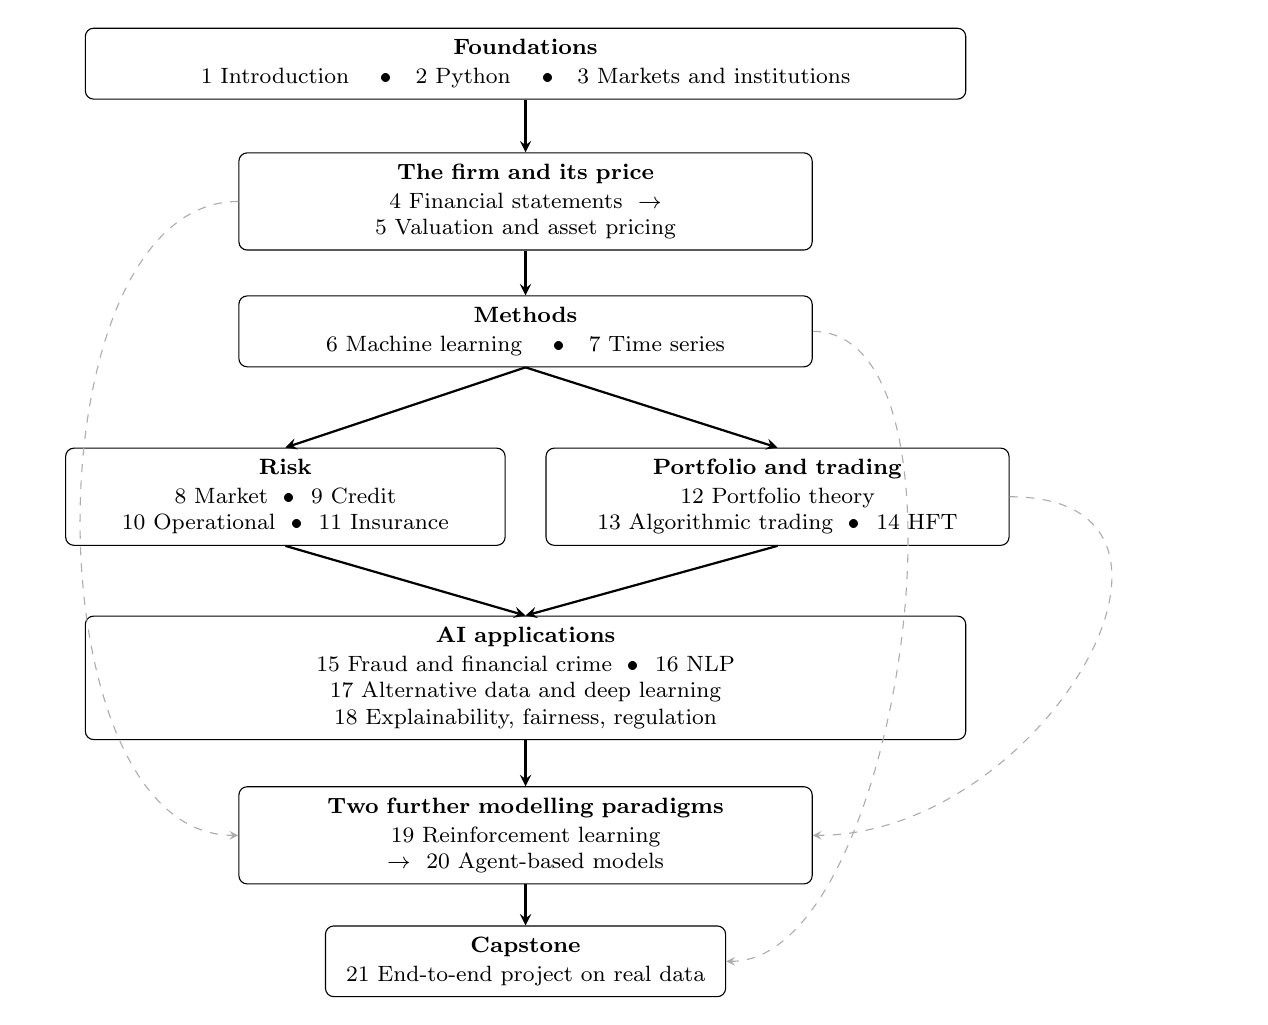
\begin{tikzpicture}[
  >=stealth,
  grp/.style={draw,rounded corners=3pt,align=center,font=\footnotesize,
              inner sep=4pt},
  main/.style={->,thick},
  back/.style={->,dashed,gray!65,thin},
]

\node[grp,text width=10.9cm] (found) at (0,0)
  {\textbf{Foundations}\\[1pt]
   1~Introduction \quad\textbullet\quad 2~Python \quad\textbullet\quad
   3~Markets and institutions};

\node[grp,text width=7.0cm] (firm) at (0,-1.75)
  {\textbf{The firm and its price}\\[1pt]
   4~Financial statements \ $\rightarrow$ \ 5~Valuation and asset pricing};

\node[grp,text width=7.0cm] (meth) at (0,-3.4)
  {\textbf{Methods}\\[1pt]
   6~Machine learning \quad\textbullet\quad 7~Time series};

\node[grp,text width=5.3cm] (risk) at (-3.05,-5.5)
  {\textbf{Risk}\\[1pt]
   8~Market \ \textbullet\ \ 9~Credit\\
   10~Operational \ \textbullet\ \ 11~Insurance};

\node[grp,text width=5.6cm] (trade) at (3.2,-5.5)
  {\textbf{Portfolio and trading}\\[1pt]
   12~Portfolio theory\\
   13~Algorithmic trading \ \textbullet\ \ 14~HFT};

\node[grp,text width=10.9cm] (apps) at (0,-7.8)
  {\textbf{AI applications}\\[1pt]
   15~Fraud and financial crime \ \textbullet\ \ 16~NLP\\
   17~Alternative data and deep learning\\
   18~Explainability, fairness, regulation};

\node[grp,text width=7.0cm] (para) at (0,-9.8)
  {\textbf{Two further modelling paradigms}\\[1pt]
   19~Reinforcement learning \ $\rightarrow$ \ 20~Agent-based models};

\node[grp,text width=4.8cm] (cap) at (0,-11.4)
  {\textbf{Capstone}\\[1pt] 21~End-to-end project on real data};

% the spine
\draw[main] (found) -- (firm);
\draw[main] (firm)  -- (meth);
\draw[main] (meth.south) -- (risk.north);
\draw[main] (meth.south) -- (trade.north);
\draw[main] (risk.south)  -- (apps.north);
\draw[main] (trade.south) -- (apps.north);
\draw[main] (apps) -- (para);
\draw[main] (para) -- (cap);

% The load-bearing reuse that crosses tiers, drawn outside the spine. These are
% deliberately unlabelled in the picture and named in the caption instead:
% labelling them here made the figure wider than the text block and forced ugly
% hyphenation inside the boxes.
\draw[back] (firm.west) to[out=180,in=180,looseness=0.85] (para.west);
\draw[back] (meth.east) to[out=0,in=0,looseness=0.7]  (cap.east);
\draw[back] (trade.east) to[out=0,in=0,looseness=1.5] (para.east);

\end{tikzpicture}
\caption{How the chapters depend on one another. Solid arrows are prerequisites.
The three dashed arrows mark the places where a later group reuses an earlier
one's machinery rather than rebuilding it: Chapter 5's option pricing returns in
Chapters 8, 9, 12, and 19; Chapter 6's models are reused by Chapter 9 and
Chapters 15 through 18 rather than retaught; and Chapter 13's execution model
returns in Chapter 19. Chapter 2 underpins every companion notebook in the book
and Chapter 21 draws on all of it, so neither is drawn with an arrow to each
dependent chapter. An instructor short of sessions can cut most safely within a
group rather than across the spine.}
\label{fig:chapter-dependencies}
\end{figure}
%%% FIGURE -- end of the block that moves

\end{document}
